%%%%%%%%%%%%%%%%%%%%%%%%%%%%%%%%%%%%%%%%%
% University/School Laboratory Report
% LaTeX Template
% Version 4.0 (March 21, 2022)
%
% This template originates from:
% https://www.LaTeXTemplates.com
%
% Authors:
% Vel (vel@latextemplates.com)
% Linux and Unix Users Group at Virginia Tech Wiki
%
% License:
% CC BY-NC-SA 4.0 (https://creativecommons.org/licenses/by-nc-sa/4.0/)
%
%%%%%%%%%%%%%%%%%%%%%%%%%%%%%%%%%%%%%%%%%

%----------------------------------------------------------------------------------------
%	PACKAGES AND DOCUMENT CONFIGURATIONS
%----------------------------------------------------------------------------------------

\documentclass[
	letterpaper, % Paper size, specify a4paper (A4) or letterpaper (US letter)
	10pt, % Default font size, specify 10pt, 11pt or 12pt
]{CSUniSchoolLabReport}

%packages
\usepackage{minted}
\setminted{breaklines}
\usepackage{import}

\addbibresource{sample.bib} % Bibliography file (located in the same folder as the template)

%----------------------------------------------------------------------------------------
%	REPORT INFORMATION
%----------------------------------------------------------------------------------------

\title{Building an Integer ALU Final Step\\ CS 3339 \\ Group: The Architects} % Report title

\author{Aaron \textsc{Reed} \& Carlo \textsc{Marroquin} \& Ryan \textsc{Bieker}} % Author name(s), add additional authors like: '\& James \textsc{Smith}'

\date{\today} % Date of the report

%----------------------------------------------------------------------------------------

\begin{document}

\maketitle % Insert the title, author and date using the information specified above

\begin{center}
	\begin{tabular}{l r}
		Instructor: & Professor \textsc{Klepetko} % Instructor/supervisor
	\end{tabular}
\end{center}

%----------------------------------------------------------------------------------------
%	OBJECTIVE
%----------------------------------------------------------------------------------------

\section{Objective}

To introduce the process and methodology of designing a new computer circuit from scratch by coding 4-bit Binary Functions And, Nand, Or, Nor, Xor, Xnor, Not, and a Shifter. 4-bit arithmetic operations Addition, Subtraction, Multiplication all including carry in and carry out circuits. The ALU functions were then integrated into a control circuit. This circuit controls user input in hexadecimal coded in to choose which ALU function output to display..

\section{Verilog Code}
To design our Verilog control Circuit we decided on Operation Codes for each module. The Operation Codes in hexadecimal are: 

\begin{table}[H]
    \centering
    \begin{tabular}{c|c}
       AND  & 0 \\
       NAND  & 1 \\
       OR & 2 \\
       NOR & 3 \\
       XOR & 4 \\
       XNOR & 5 \\
       NOT & 6 \\
       SHIFT & 7 \\
       ADD & 8 \\
       SUBTRACT & 9 \\
       MULTIPLY & A 
    \end{tabular}
    \caption{Operation Codes for ALU Modules}
    \label{tab:my_label}
\end{table}

\section{Control Design}
\begin{center}
    \inputminted{octave}{verilog/control/control.v}
\end{center}
\section{Control Testbench}
\begin{center}
    \inputminted{octave}{verilog/control/control_test.v}
\end{center}

\section{Waveforms}
Waveforms with an X and Y input, with 2 test cases for each operation.

    

\section{AND}
\begin{figure}[H] % [H] forces the figure to be placed exactly where it appears in the text
    %\centering % Horizontally center the figure
    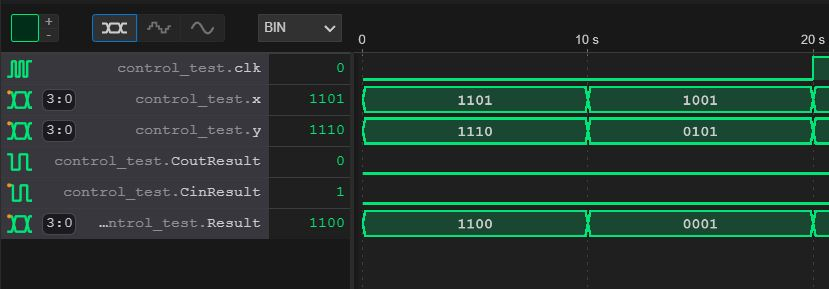
\includegraphics[width=\textwidth]{figures/and.JPG} % Include the figure
    \caption{The AND Waveform.}
\end{figure}
\section{NAND}
\begin{figure}[H] % [H] forces the figure to be placed exactly where it appears in the text
    %\centering % Horizontally center the figure
    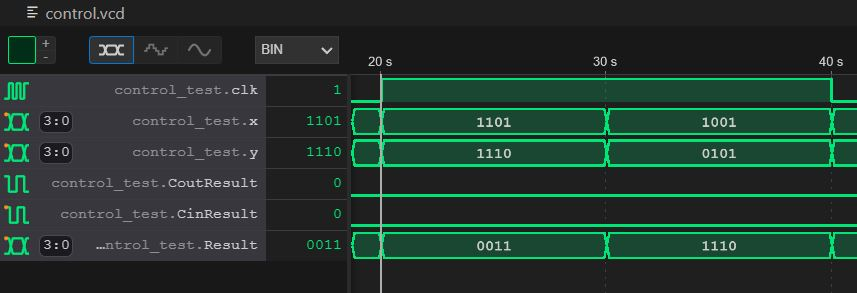
\includegraphics[width=\textwidth]{figures/nand.JPG} % Include the figure
    \caption{The NAND waveform.}
\end{figure}
\section{OR}
\begin{figure}[H] % [H] forces the figure to be placed exactly where it appears in the text
    %\centering % Horizontally center the figure
    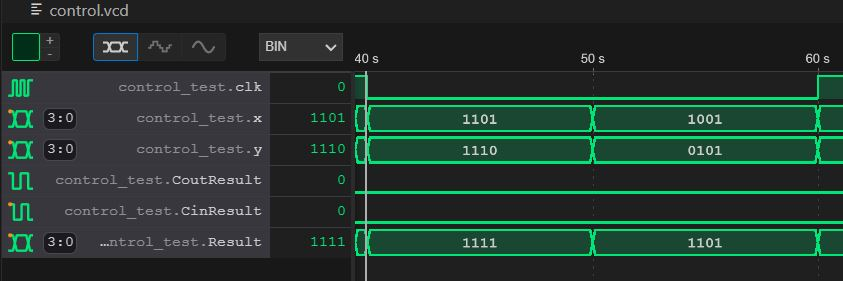
\includegraphics[width=\textwidth]{figures/or.JPG} % Include the figure
    \caption{The OR waveform.}
\end{figure}
\section{NOR}
\begin{figure}[H] % [H] forces the figure to be placed exactly where it appears in the text
    %\centering % Horizontally center the figure
    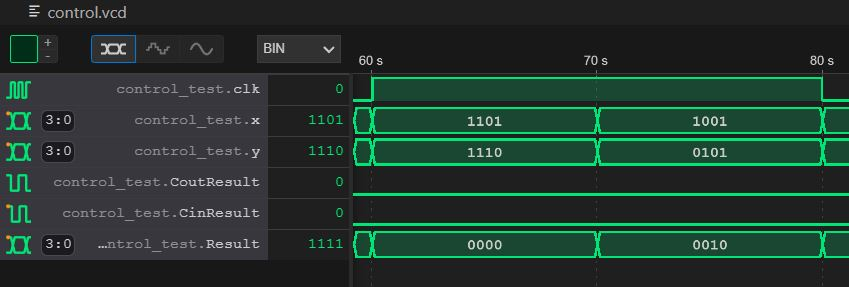
\includegraphics[width=\textwidth]{figures/nor.JPG} % Include the figure
    \caption{The NOR waveform.}
\end{figure}
\section{XOR}
\begin{figure}[H] % [H] forces the figure to be placed exactly where it appears in the text
    %\centering % Horizontally center the figure
    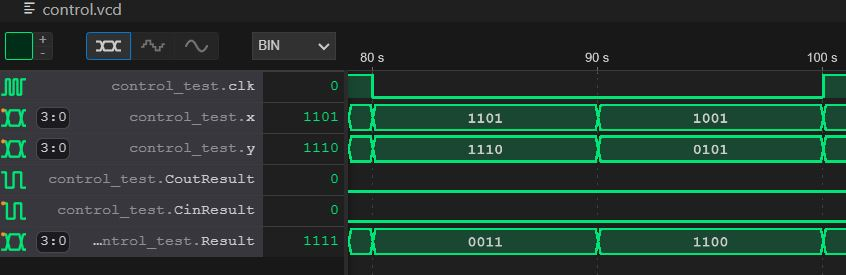
\includegraphics[width=\textwidth]{figures/xor.JPG} % Include the figure
    \caption{The XOR waveform.}
\end{figure}
\section{XNOR}
\begin{figure}[H] % [H] forces the figure to be placed exactly where it appears in the text
    %\centering % Horizontally center the figure
    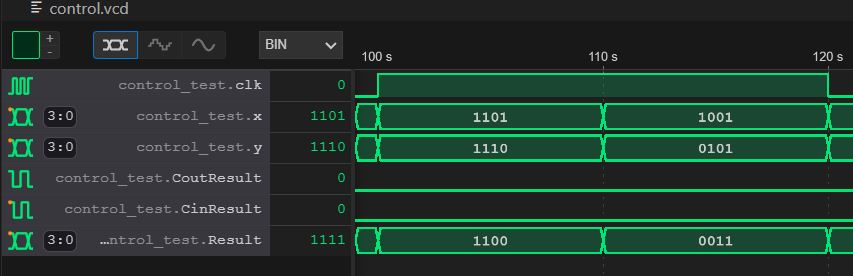
\includegraphics[width=\textwidth]{figures/xnor.JPG} % Include the figure
    \caption{The XNOR waveform.}
\end{figure}
\section{NOT}
\begin{figure}[H] % [H] forces the figure to be placed exactly where it appears in the text
    %\centering % Horizontally center the figure
    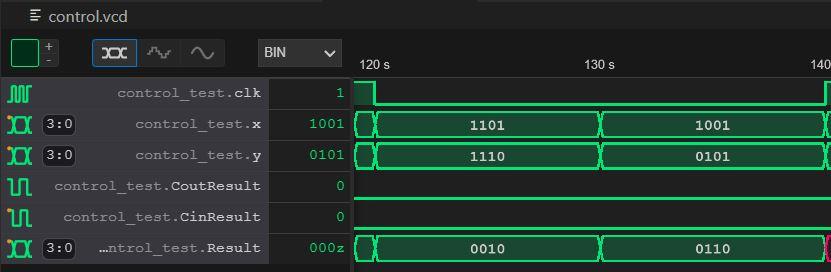
\includegraphics[width=\textwidth]{figures/not.JPG} % Include the figure
    \caption{The NOT waveform.}
\end{figure}
\section{SHIFT}
\begin{figure}[H] % [H] forces the figure to be placed exactly where it appears in the text
    %\centering % Horizontally center the figure
    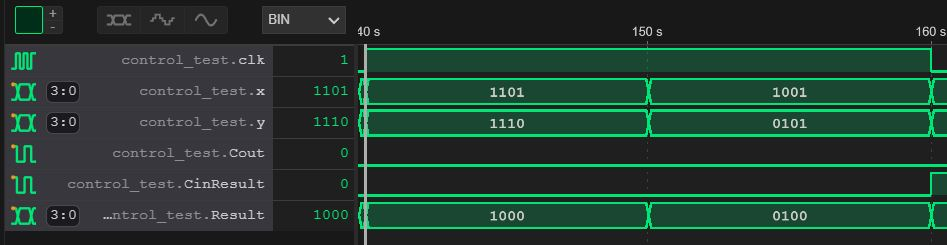
\includegraphics[width=\textwidth]{figures/shift.JPG} % Include the figure
    \caption{The SHIFT waveform.}
\end{figure}
\section{ADD}
\begin{figure}[H] % [H] forces the figure to be placed exactly where it appears in the text
    %\centering % Horizontally center the figure
    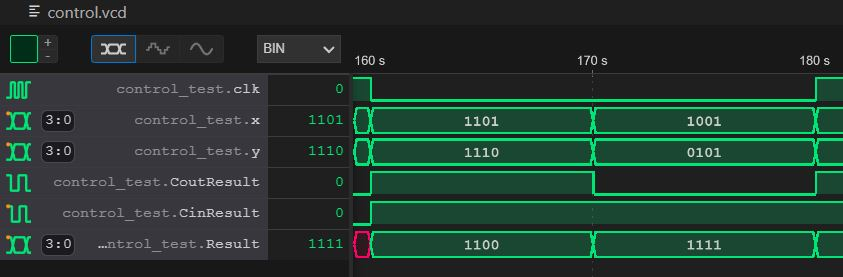
\includegraphics[width=\textwidth]{figures/add.JPG} % Include the figure
    \caption{The ADD waveform.}
\end{figure}
\section{SUB}
\begin{figure}[H] % [H] forces the figure to be placed exactly where it appears in the text
    %\centering % Horizontally center the figure
    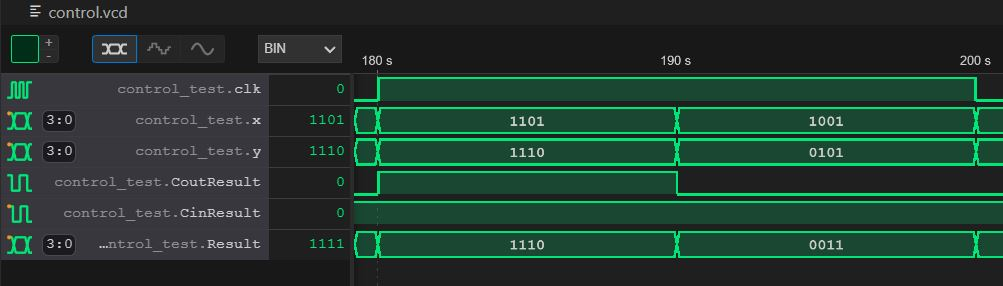
\includegraphics[width=\textwidth]{figures/sub.JPG} % Include the figure
    \caption{The SUB waveform.}
\end{figure}
\section{MULT}
\begin{figure}[H] % [H] forces the figure to be placed exactly where it appears in the text
    %\centering % Horizontally center the figure
    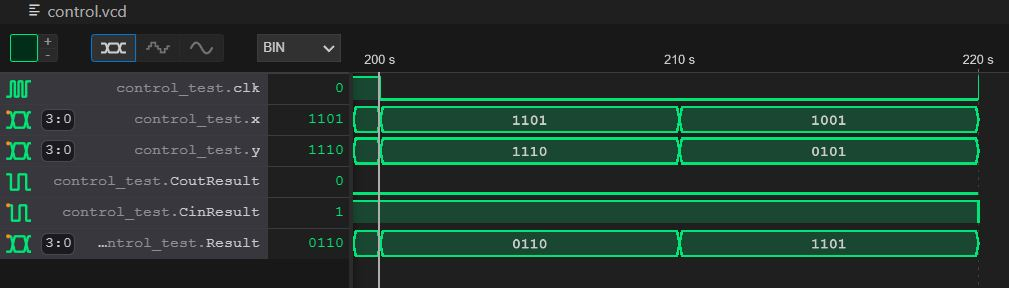
\includegraphics[width=\textwidth]{figures/mult.JPG} % Include the figure
    \caption{The MULT waveform.}
\end{figure}

\section{Conclusion}
In order to create our 4-bit modules in Verilog, we had to determine how to store 4-bit numbers in registers and wires. Addition was the most straightforward to code with Carry-In and Carry-Out values.  In our multiplication module, we found that the product of two 4-bit numbers needed to be 8-bits in order to properly implement the Carry-Out of the module. The multiplication module gave us the most trouble as we couldn’t decide what size the output product should be. The logic gates were quick to get through using 4-bit values as they are built into the Verilog code as operators. We imported each ALU function and connected them to a control circuit. From the control circuit, we were able to have a user input to choose the desired ALU function. From here, the control circuit would select the output for the user chosen function in hexadecimal coded in after running every function. Each operation was run in two test cases.
\end{document}
